\documentclass[tikz,border=15pt]{standalone}
\usepackage{helvet}
\renewcommand{\familydefault}{\sfdefault}
\usetikzlibrary{positioning, fit, arrows.meta, backgrounds, calc}

\definecolor{navyblue}{HTML}{0F172A}
\definecolor{copper}{HTML}{B87333}
\definecolor{bglight}{HTML}{F8FAFC}

\begin{document}
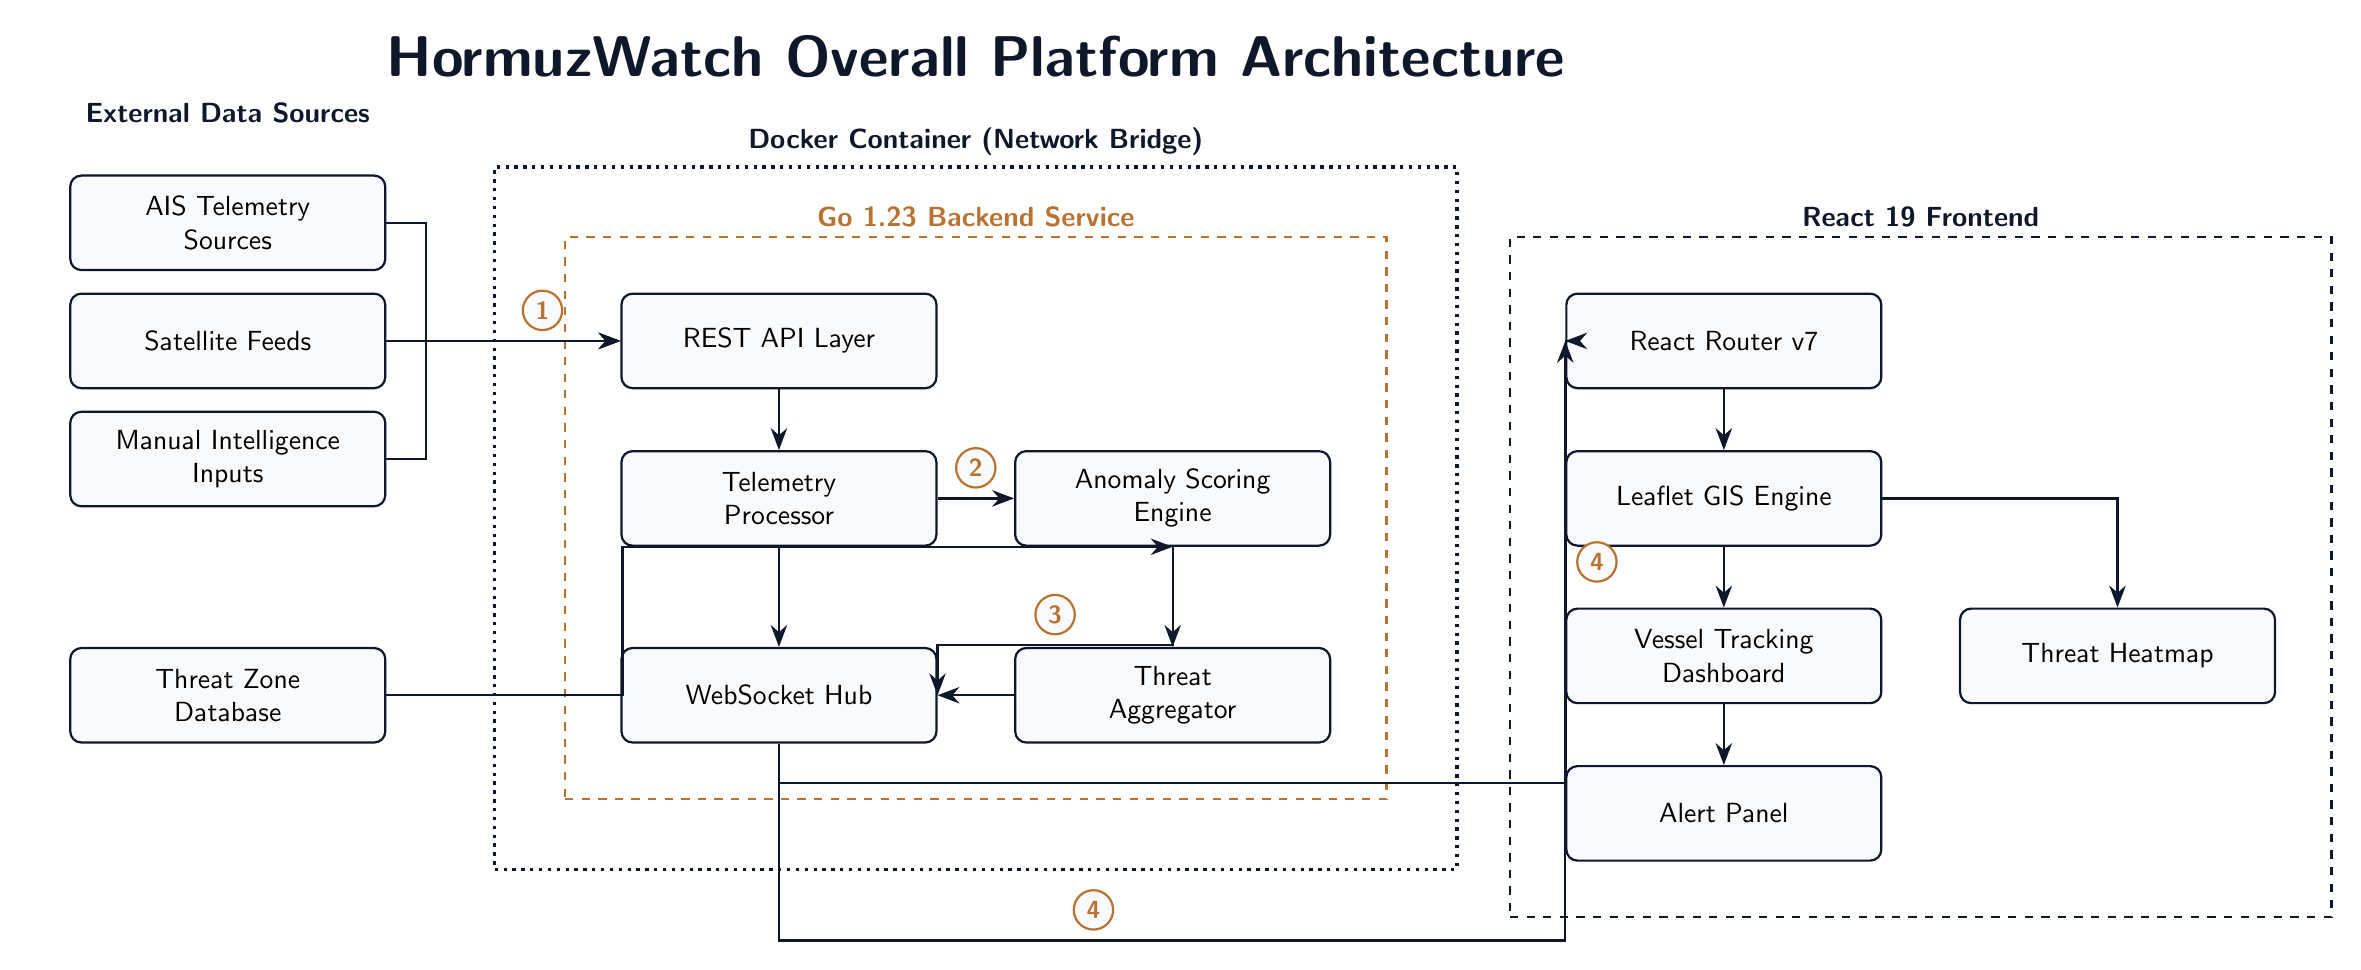
\begin{tikzpicture}[
    font=\sffamily,
    box/.style={rectangle, draw=navyblue, thick, fill=bglight, rounded corners, minimum width=4cm, minimum height=1.2cm, align=center},
    container/.style={rectangle, draw=copper, thick, dashed, inner sep=20pt},
    frontcontainer/.style={rectangle, draw=navyblue, thick, dashed, inner sep=20pt},
    arrow/.style={-{Stealth[scale=1.2]}, thick, navyblue},
    stage/.style={circle, draw=copper, fill=bglight, thick, inner sep=1pt, minimum size=0.5cm, font=\bfseries\small, text=copper}
]

% ==================== LEFT SIDE: SOURCES ====================
\node[box] (ais) at (0, 3) {AIS Telemetry\\Sources};
\node[box] (sat) at (0, 1.5) {Satellite Feeds};
\node[box] (manual) at (0, 0) {Manual Intelligence\\Inputs};
\node[box] (threatdb) at (0, -3) {Threat Zone\\Database};

\node[fit=(ais) (sat) (manual) (threatdb), inner sep=15pt] (sources_fit) {};
\node[above, font=\bfseries\color{navyblue}] at (sources_fit.north) {External Data Sources};

% ==================== CENTER: GO BACKEND ====================
\node[box] (rest) at (7, 1.5) {REST API Layer};
\node[box] (telemetry) at (7, -0.5) {Telemetry\\Processor};
\node[box] (anomaly) at (12, -0.5) {Anomaly Scoring\\Engine};
\node[box] (hub) at (7, -3) {WebSocket Hub};
\node[box] (aggregator) at (12, -3) {Threat\\Aggregator};

% Backend Container
\node[fit=(rest) (telemetry) (anomaly) (hub) (aggregator), container] (backend) {};
\node[above, font=\bfseries\color{copper}] at (backend.north) {Go 1.23 Backend Service};

% Docker Network Bridge (outer container)
\node[fit=(backend), rectangle, draw=navyblue, very thick, dotted, inner sep=25pt] (docker) {};
\node[above, font=\bfseries\color{navyblue}] at (docker.north) {Docker Container (Network Bridge)};

% ==================== RIGHT SIDE: REACT FRONTEND ====================
\node[box] (router) at (19, 1.5) {React Router v7};
\node[box] (gis) at (19, -0.5) {Leaflet GIS Engine};
\node[box] (dashboard) at (19, -2.5) {Vessel Tracking\\Dashboard};
\node[box] (heatmap) at (24, -2.5) {Threat Heatmap};
\node[box] (alert) at (19, -4.5) {Alert Panel};

% Frontend Container
\node[fit=(router) (gis) (dashboard) (heatmap) (alert), frontcontainer] (frontend) {};
\node[above, font=\bfseries\color{navyblue}] at (frontend.north) {React 19 Frontend};

% ==================== ARROWS & FLOW ====================
% Sources to Backend
\draw[arrow] (ais.east) -- ++(0.5,0) |- (rest.west);
\draw[arrow] (sat.east) -- ++(0.5,0) |- (rest.west) node[pos=0.8, above] {\tikz{\node[stage] {1};}};
\draw[arrow] (manual.east) -- ++(0.5,0) |- (rest.west);
\draw[arrow] (threatdb.east) -- ++(3,0) |- (anomaly.south);

% Inside Backend
\draw[arrow] (rest.south) -- (telemetry.north);
\draw[arrow] (telemetry.east) -- (anomaly.west) node[midway, above] {\tikz{\node[stage] {2};}};
\draw[arrow] (anomaly.south) -- (aggregator.north);
\draw[arrow] (aggregator.west) -- (hub.east);
\draw[arrow] (telemetry.south) -- (hub.north);
\draw[arrow] (anomaly.south) |- ++(0,-1.25) -| (hub.east) node[pos=0.25, above] {\tikz{\node[stage] {3};}};

% Backend to Frontend
\draw[arrow] (hub.south) -- ++(0,-0.5) -| ++(10,0) |- (router.west) node[pos=0.25, right] {\tikz{\node[stage] {4};}};
% Let's fix the route from Hub to Frontend:
\draw[arrow] (hub.south) |- ++(0,-2.5) -| (router.west) node[pos=0.2, above] {\tikz{\node[stage] {4};}};

% Inside Frontend
\draw[arrow] (router.south) -- (gis.north);
\draw[arrow] (gis.south) -- (dashboard.north);
\draw[arrow] (gis.east) -| (heatmap.north);
\draw[arrow] (dashboard.south) -- (alert.north);

% ==================== TITLE ====================
\node[above=1cm of docker.north, font=\huge\bfseries\color{navyblue}] {HormuzWatch Overall Platform Architecture};

\end{tikzpicture}
\end{document}
